\subsection{How does an external magnetic field affect an atom in LS-coupling? Describe the Zeeman effect without accounting for the nucleus.}


\paragraph{LS-kobling:} I atomer større end hydrogen kan hvert atoms baneimpulsmoment og spin koble sammen, hvilket giver et energiskifte i forhold til den forventede værdi baseret på Schrödingerligningen.

For lettere atomer er koblingen mellem elektronernes baneimpulsmomenter og spin indbyrdes stærkere end koblingen mellem en enkelt elektronens baneimpulsmoment og spin, hvorved energiskiftet kommer til at være i LS-koblings regimet, hvor $\Vec{J} = \Vec{L} + \Vec{S}$, hvor $\Vec{L} = \sum_i \Vec{l}_i$ og $\Vec{S} = \sum_i \Vec{s}_i$ (i stedet for $\Vec{J} = \sum_i \Vec{j}_i$, hvor $\Vec{j}_i = \Vec{l}_i + \Vec{s}_i$, hvilket er jj-koblingings regimet). Dermed har vi fået introduceret et nyt impulsmoment, det totale elektronimpulsmoment $\Vec{J} = \Vec{L} + \Vec{S}$, hvilket altså kendes som LS-koblingen. Energiskiftet for denne er
\begin{align}
    E_{HF} &= \frac{\beta}{2} \left\{J(J+1) - L(L+1) - S(S+1)\right\} \: ,
\end{align}
hvor $\beta \propto \mu_B^2$ er finstrukturkonstanten.


\paragraph{Zeemaneffekten:} Idet atomer opfører sig som magnetiske dipoler, da vil man observere et energiskift, hvis atomet indsættes i et eksternt magnetisk felt. Energiskiftet grundet vekselvirkningen mellem atomets dipolmoment og det eksterne magnetfelt vil løfte udartetheden (eng. the degeneracy) af tilstanden, idet man i LS-koblingen får en opsplitning i $M_J$.


\paragraph{Zeemaneffekten med LS-kobling:} Det totale magnetiske dipolmoment for et atom er givet som summen af dipolmomentet grundet spin og grundet baneimpulsmomentet
\begin{align}
    \Vec{\mu}_J &= \Vec{\mu}_L + \Vec{\mu}_S = - \frac{\mu_B}{\hbar} \left( g_L \Vec{L} + g_S \Vec{S} \right) \: ,
\end{align}
hvor $\mu_B = e\hbar/(2m_e)$ er Bohrmagnetronen, og $g_L \simeq 1$ og $g_S \simeq 2$ er Landé g-faktorer for hhv. baneimpulsmomentet og spinet.

Et atoms interaktion med et eksternt magnetfelt beskrives ved Hamiltonoperatoren
\begin{align} \label{eq:Q15_StartudtrykForHamiltonForZeemaneffekten}
    H_{ZE} = -\braket{\Vec{\mu}_J} \cdot \Vec{B} \: ,
\end{align}
hvor $\braket{\Vec{\mu}_J}$ er projektionen af $\Vec{\mu}_J$ ind langs $\Vec{J}$ -- dette kan ses på \cref{fig:Q15_ZeemanEffectInThePresenceOfSpin}
-- hvilken skal benyttes, da denne er en middelværdi af $\Vec{\mu}_J$ ($\Vec{\mu}_J$ præciserer omkring $\braket{\Vec{\mu}_J}$), og $\braket{\Vec{\mu}_J}$ er velbeskrevet i basen $\ket{L \: S \: J \: M_J}$, hvilket $\Vec{\mu}_J$ ikke er. Denne basis benyttes idet, at vi arbejder med LS-kobling ($E_{ZE} \ll E_{SO}$), hvorfor også interaktionen i \cref{eq:Q15_StartudtrykForHamiltonForZeemaneffekten} kan ses som værende en perturbation til finstrukturen benyttende LS-kobling.

\begin{figure}[!h]
    \centering
    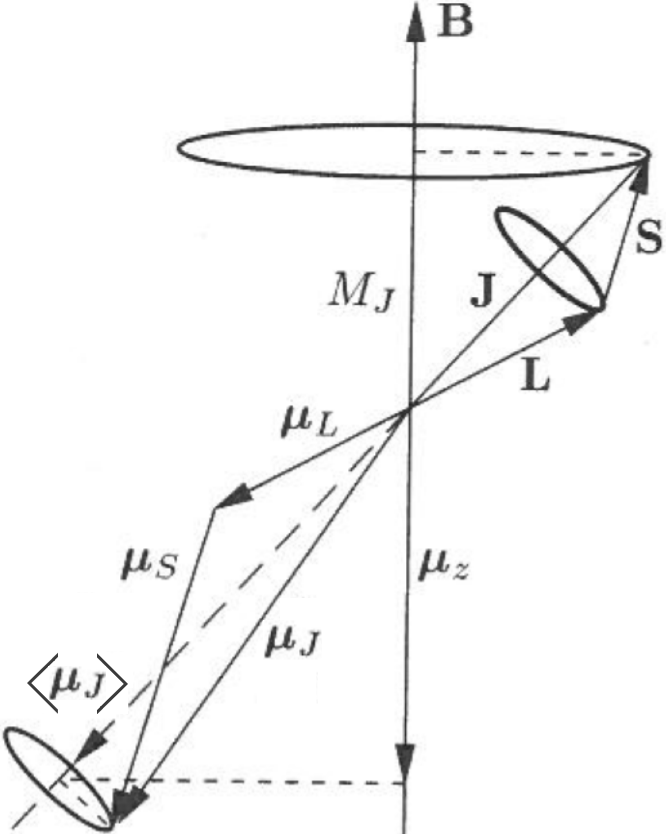
\includegraphics[width=0.4\textwidth]{Q15/images/ZeemanEffectWithLSCoupling.PNG}
    \caption{Det totale dipolmoment $\Vec{\mu}_J = \Vec{\mu}_L + \Vec{\mu}_S$, fra det magnetiske dipolmoment fra baneimpulsmomentet og af det fra spinet, og dets projektion langs $\Vec{J}$, $\braket{\Vec{\mu}_J}$ (hvilket er en middelværdi og ikke en forventningsværdi).}
    \label{fig:Q15_ZeemanEffectInThePresenceOfSpin}
\end{figure}

Projektionen $\braket{\Vec{\mu}_J}$ findes ved
\begin{align}
    \braket{\Vec{\mu}_J} &= \left(\Vec{\mu}_J \cdot \Hat{J}\right) \Hat{J} = \frac{\Vec{\mu}_J \cdot \Vec{J}}{\abs{\Vec{J} \,}^2} \Vec{J} = - \frac{\mu_B}{\hbar} \left( g_L \frac{\Vec{L} \cdot \Vec{J}}{\abs{\Vec{J} \,}^2} + g_S \frac{\Vec{S} \cdot \Vec{J}}{\abs{\Vec{J} \,}^2} \right) \Vec{J} \: ,
\end{align}
hvor $\Hat{J} = \Vec{J}/|\Vec{J}|$. Derved bliver Hamiltonoperatoren fra \cref{eq:Q15_StartudtrykForHamiltonForZeemaneffekten}, idet $\Vec{B} = B\Hat{z}$,
\begin{align}
    H_{ZE} &= -\left\{- \frac{\mu_B}{\hbar} \left( g_L \frac{\Vec{L} \cdot \Vec{J}}{\abs{\Vec{J} \,}^2} + g_S \frac{\Vec{S} \cdot \Vec{J}}{\abs{\Vec{J} \,}^2} \right) \Vec{J} \right\} \cdot \Vec{B} = \frac{\mu_B}{\hbar} \left( \frac{\Vec{L} \cdot \Vec{J}}{\abs{\Vec{J} \,}^2} + 2\frac{\Vec{S} \cdot \Vec{J}}{\abs{\Vec{J} \,}^2} \right) B J_z \: ,
\end{align}
hvor det er blevet brugt, at $g_L \simeq 1$ og $g_S \simeq 2$, hvormed energiskiftet grundet Zeemaneffekten bliver
\begin{align} \label{eq:Q15_EnergyZeemanInLSCouplingStart}
    E_{ZE} &= \braket{H_{ZE}} = \frac{\mu_B}{\hbar} \left( \frac{\braket{\Vec{L} \cdot \Vec{J}}}{\hbar^2 J(J+1)} + 2 \frac{\braket{\Vec{S} \cdot \Vec{J}}}{\hbar^2 J(J+1)} \right) B \braket{J_z} \: .
\end{align}

Forventningsværdien af $\braket{\Vec{L} \cdot \Vec{J}}$ og $\braket{\Vec{S} \cdot \Vec{J}}$ findes ved at $\Vec{J} = \Vec{L} + \Vec{S}$, så
\begin{align}
    \Vec{S} &= \Vec{J} - \Vec{L} \Rightarrow \Vec{S}^2 = \Vec{J}^2 + \Vec{L}^2 - 2\Vec{L} \cdot \Vec{J} \nonumber\\
    \Rightarrow \braket{\Vec{L} \cdot \Vec{J}} &= \frac{1}{2} \left(\braket{\Vec{J}^2} + \braket{\Vec{L}^2} - \braket{\Vec{S}^2}\right) = \frac{\hbar^2}{2} \left\{J(J+1) + L(L+1) - S(S+1)\right\} \: , \\
    \Vec{L} &= \Vec{J} - \Vec{S} \Rightarrow \Vec{L}^2 = \Vec{J}^2 + \Vec{S}^2 - 2\Vec{S} \cdot \Vec{J} \nonumber\\
    \Rightarrow \braket{\Vec{S} \cdot \Vec{J}} &= \frac{1}{2} \left(\braket{\Vec{J}^2} + \braket{\Vec{S}^2} - \braket{\Vec{L}^2}\right) = \frac{\hbar^2}{2} \left\{J(J+1) + S(S+1) - L(L+1)\right\} \: ,
\end{align}
hvorved vi får \cref{eq:Q15_EnergyZeemanInLSCouplingStart} til at blive
\begin{align}
    E_{ZE} &= \frac{\mu_B}{\hbar^3 J(J+1)} \frac{\hbar^2}{2}\left\{3J(J+1) - L(L+1) + S(S+1)\right\} B \braket{J_z} \nonumber\\
    &= \frac{\mu_B}{\hbar} \frac{3J(J+1) + S(S+1) - L(L+1)}{2J(J+1)} B \braket{J_z} \nonumber\\
    &= \frac{\mu_B}{\hbar} \frac{3}{2} + \frac{S(S+1) - L(L+1)}{2J(J+1)} B \hbar M_J \nonumber\\
    &= g_J M_J \mu_B B_z \: , \quad \text{hvor} \quad g_J = \frac{3}{2} + \frac{S(S+1) - L(L+1)}{2J(J+1)} \: .
\end{align}



\paragraph{Normal og unormal Zeemaneffekt:} Man taler om to former for Zeemanopdeling, normal og unormal, hvilket skyldes henholdsvis singlet- og triplet-tilstande.

\begin{figure}[!h]
    \centering
    \begin{subfigure}[t]{0.46\textwidth}
        \centering
        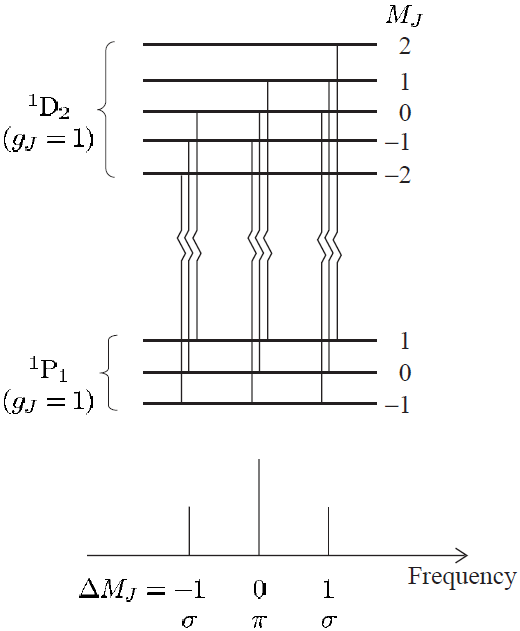
\includegraphics[width=\columnwidth]{Q15/images/NormalZeemanEffect.PNG}
        \caption{Den normale Zeemaneffekt (eng. normal Zeeman effect). $S = 0$.}
        \label{fig:Q15_NormalZeemanEffect}
    \end{subfigure}
    \hfill
    \begin{subfigure}[t]{0.46\textwidth}
        \centering
        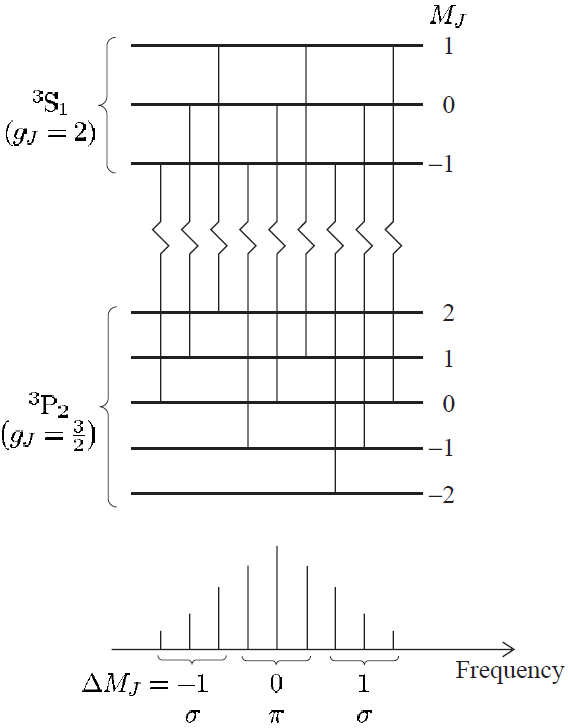
\includegraphics[width=\columnwidth]{Q15/images/AnomalousZeemanEffect.PNG}
        \caption{Den unormale Zeemaneffekt (eng. anomalous Zeeman effect). $S \ne 0$.}
        \label{fig:Q15_AnomalousZeemanEffect}
    \end{subfigure}
    \caption{}
    \label{fig:Q15_TypesOfZeemanEffect}
\end{figure}

For singlets er $S = 0$, hvorfor $\Vec{J} = \Vec{L}$, og derved bliver $g_J = 1$, hvorfor der ikke er behov for at projicere dipolmomneterne, da $\Vec{\mu}_J = \braket{\Vec{\mu}_J}$. Derved vil der være den samme Zeemanopdeling mellem $M_J$ stadierne. Overgange mellem singlettilstande kaldes \emph{normal Zeemaneffekt} (eng. noraml Zeeman effect), da navnet stammer fra, at man ikke var bekendt med spin, hvorfor en tilstand med $S = 0 \Rightarrow \Vec{J} = \Vec{L}$ vil opføre sig, som man forventer, hvis man blot formodede, at atomer havde baneimpulsmomentet $\Vec{L}$ som deres totale impulsmoment. Denne kan ses på \cref{fig:Q15_NormalZeemanEffect}. Overgangene med $\Delta M_J = \pm 1$ har frekvenser, som er skiftet med $\pm \mu_B B / h$ mht. $\Delta M_J = 0$ overgangen\footnote{$1/h$ kommer fra omregningen mellem energi og frekvens.}.

Den \emph{unormale Zeemaneffekt} ($S \ne 0$) opstår grundet overgange mellem triplettilstande i atomer med (blandt andet) to uparrede valenselektroner\footnote{Den unormale Zeemaneffekt opstår generelt i alle tilfælde, hvor der opstår en opsplitning grundet et eksternt magnetfelts vekselvirkning med atomet, og $S \ne 0$.}. Det observerede mønster, \cref{fig:Q15_AnomalousZeemanEffect}, afhænger af $g_J$ og af $J$ for de øvre og nedre niveauer, da ???.

I både den normale og den unormale Zeemaneffekt har $\pi$-overgangene ($\Delta M_J = 0$) og $\sigma$-overgangene ($\Delta M_J = \pm 1$) samme polarisation som i den klassiske model beskrevet øverst oppe i denne disposition.\\


Et eksempel på en opdeling grundet Zeemaneffekten i LS-kobling for en tilstand med $J = 2$ kan ses på \cref{fig:Q15_ZeemanWithLSCouplingSplittings}, hvor den splitter til $2M_J + 1$ tilstande med $M_J \in [-2,\, -1,\, 0,\, 1,\, 2]$.

\begin{figure}[!h]
    \centering
    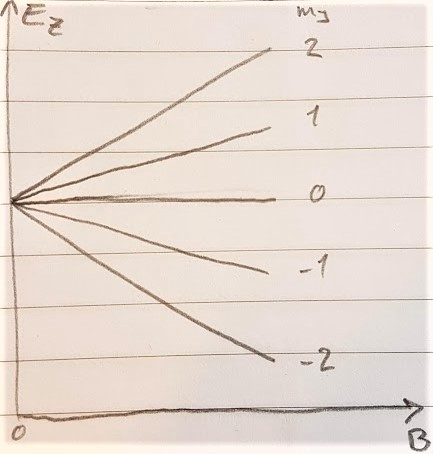
\includegraphics[width=0.5\textwidth]{Q15/images/ZeemanEffectWithLSCouplingSplitting.jpg}
    \caption{Eksempel på opdeling grundet stigende B-felt.}
    \label{fig:Q15_ZeemanWithLSCouplingSplittings}
\end{figure}